\section{Classical model of light}\label{sec:1-classical-model-of-light}
In this section we study coherence and optical fluctuations within the classical theory, and then highlight phenomena that cannot be fully explained in classical terms.
\subsection{Young experiment and Mach-Zehnder interferometer}\label{subsec:1-young-exp}
Suppose we have a monochromatic beam of light incident on an opaque screen with two small holes, $A$ and $B$. After passing through the holes, the light diffracts and, at a sufficiently large distance, an interference pattern is observed on a photographic plate.
\begin{figure}[H]\label{1-young}       
    \centering            
    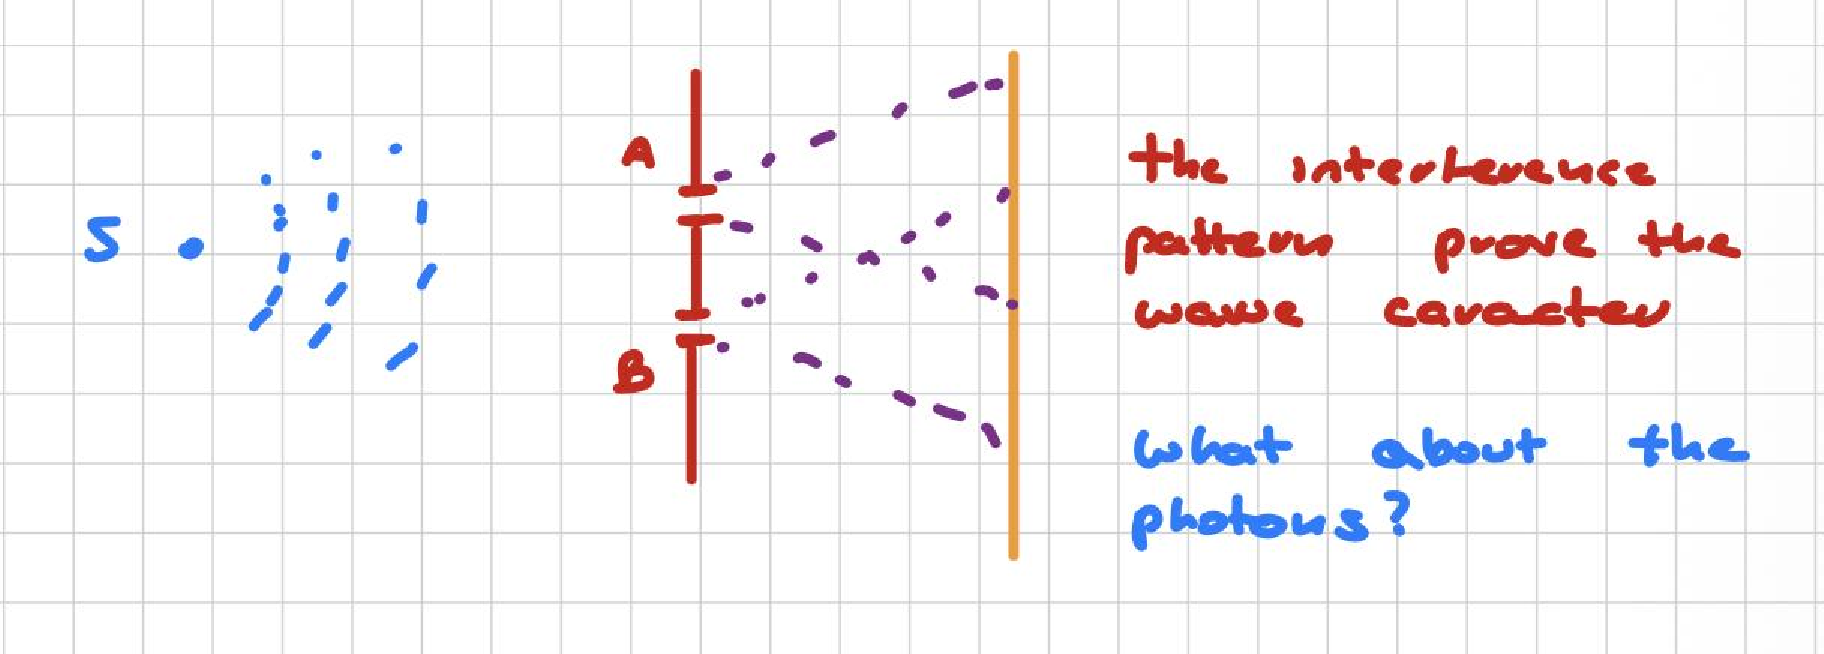
\includegraphics[width=0.8\textwidth]{images_in_pdf/1-/Grafico_1.pdf} 
\end{figure}

Now let us gradually decrease the light intensity so that, effectively, only one photon is sent at a time. By increasing the exposure time, the same interference pattern is still built up on the screen, one detection event after another. 

Now suppose we close one of the two holes, so that we obtain the diffraction pattern associated with hole $A$ or hole $B$ alone.
\begin{figure}[H]       
    \centering            
    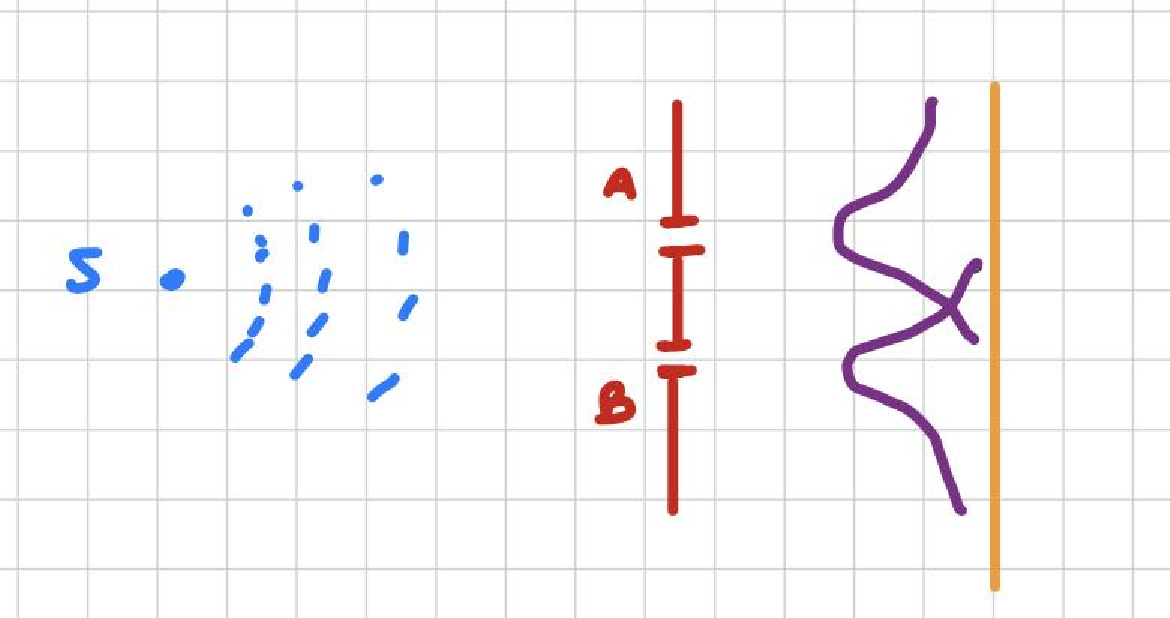
\includegraphics[width=0.8\textwidth]{images_in_pdf/1-/Grafico_2.pdf} 
\end{figure}

If we assume that $50\%$ of the photons go through $A$ and the remaining $50\%$ go through $B$, then we would expect the observed distribution to be the sum of the two single-slit diffraction patterns. However, this is not what happens in the double-slit experiment: \hl{the presence of both slits together produces an \textbf{interference pattern} that cannot be reproduced by simply adding the two single-slit intensities.} In classical language, one would say that the alternatives $A$ and $B$ are not sufficient to describe the phenomenon. In quantum mechanics, \hl{the correct description is a coherent \textbf{superposition} of the two paths rather than a classical mixture.}

We now modify the experiment by introducing a Mach-Zehnder interferometer, which is composed of:
\begin{itemize}
    \item two semi-transparent mirrors, $S_1$ and $S_4$;
    \item two normal mirrors, $S_2$ and $S_3$;
    \item two detectors, $D_1$ and $D_2$.
\end{itemize}
\begin{figure}[H]\label{1-mach-zehnder}   
    \centering            
    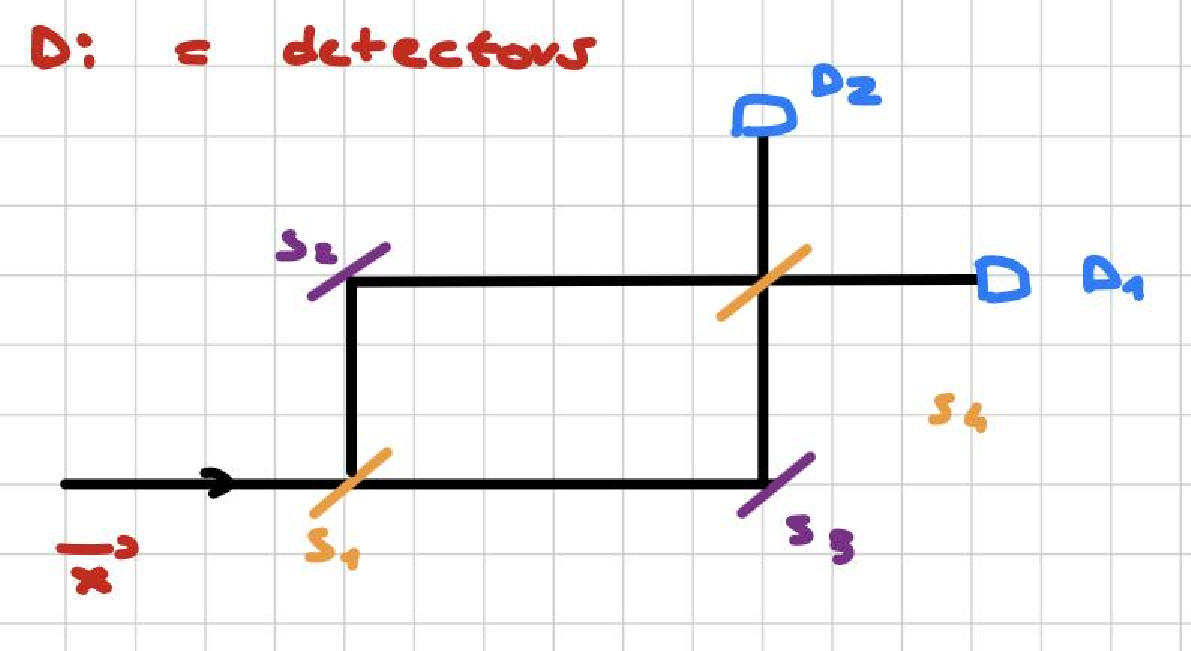
\includegraphics[width=0.8\textwidth]{images_in_pdf/1-/Grafico_3.pdf} 
\end{figure}

The beam is split at $S_1$ into two paths, reflected by $S_2$ and $S_3$, and finally recombined at $S_4$. If the interferometer is perfectly balanced, each arm carries half of the incident field amplitude and each detector receives $25\%$ of total radiation.
\begin{itemize}
     \item Path A
     \[S_1 \to S_2 \to S_4 \hspace{1.5cm}\frac{1}{2}\cdot  E_0 \cdot \cos(\omega t + \phi_1)\]
     \item Path B
     \[S_1 \to S_3 \to S_4 \hspace{1.5cm} \frac{1}{2} E_0 \cdot \cos(\omega t + \phi_2)\]
\end{itemize}

Denoting the phases accumulated along the two paths by $\phi_1$ and $\phi_2$, the two contributions at the output interfere and we measure the time average on a sufficiently long period of time:
\begin{itemize}
\item Intensity incident on $S_1$: 
\[C \cdot E^2(x,t) \implies I = C \cdot E_0^2 \cdot \braket{\cos^2(\omega t)} \propto \frac{1}{2} E_0^2\]
Where $C$ is a normalization constant.
\item Intensity incident on $D_1$:
\[I_{D_1} = C \cdot E_0^2 \cdot \braket{[\cos(\omega t + \phi_1)+\cos(\omega t + \phi_2)]^2}
= \frac{1}{2} I_0 \cdot \biggr(1+\cos(\Delta \phi)\biggr) \hspace{1cm} \Delta \phi = \phi_1-\phi_2\]
\end{itemize}

But the total intensity is given by:
\[I_{tot} = I_{D_1} + I_{D_2}\]

So we obtain:
\begin{equation}
\begin{cases}
    I_{D_1} = \frac{I_0}{2}\bigl(1+\cos\Delta\phi\bigr)\\
    I_{D_2} = \frac{I_0}{2}\bigl(1-\cos\Delta\phi\bigr)
\end{cases}
\end{equation}

where $I_0$ is the input intensity. Equivalently,
\begin{equation}
\begin{cases}
I_{D_1}=I_0\cos^2\!\left(\frac{\Delta\phi}{2}\right)\\
I_{D_2}=I_0\sin^2\!\left(\frac{\Delta\phi}{2}\right)
\end{cases}
\end{equation}

Thus, by changing the relative phase, one can continuously modulate the output intensities and obtain either constructive or destructive interference. In particular, if $\Delta\phi=0$, all the intensity exits through one detector, while the other one receives no light.

If we insert a thin glass plate in one arm of the interferometer, the optical path length changes and a phase shift is introduced. For a plate of thickness $d$ and refractive index $n$, the additional phase is
\[
\delta\phi = k_0(n-1)d = \frac{2\pi}{\lambda_0}(n-1)d,
\]

where $\lambda_0$ is the wavelength in vacuum. Even a small change in phase is enough to redistribute the counts between $D_1$ and $D_2$.

\question{Now send one photon at a time through the interferometer: should the counts at $D_1$ and $D_2$ be equal?}
{The answer is no. Because the two probability amplitudes interfere, the detection probabilities still depend on the relative phase $\Delta\phi$.} 


\calloutwarn{In the quantum description, the photon cannot be assigned a definite classical trajectory through path $A$ or path $B$. Instead, the state is described by a coherent superposition of the two paths, which is what gives rise to interference.}

\question{Returning to the Young experiment, suppose we place two detectors after the two slits $A$ and $B$: \textbf{should they click together?}}{%
\begin{figure}[H]       
    \centering            
    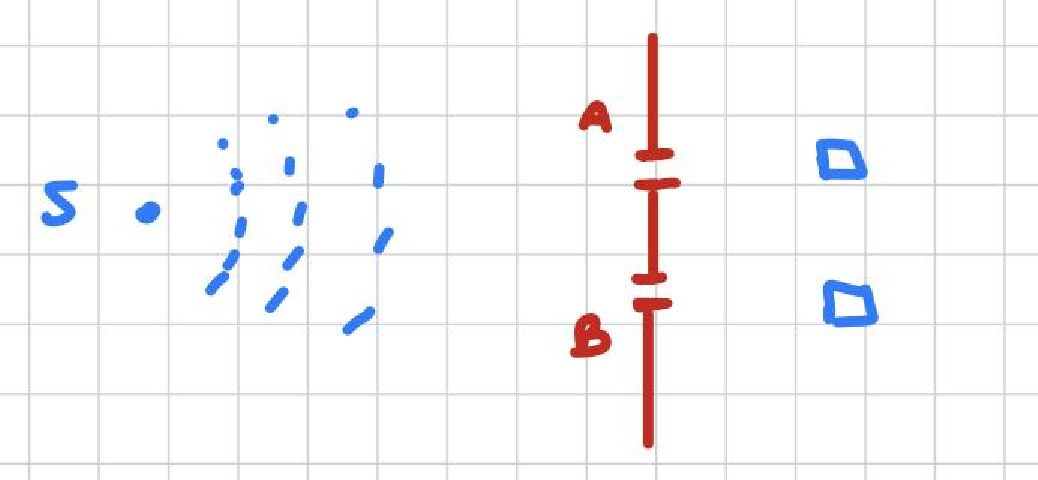
\includegraphics[width=0.5\textwidth]{images_in_pdf/1-/Grafico_4.pdf} 
\end{figure}

The answer is no. A single photon cannot be split into two independent detection events. Repeating the experiment many times, one finds that each photon is detected by one detector only and, on average, the counts are distributed according to the measurement probabilities $50 \%$  clicks on $D_1$ and  $50 \%$ clicks on $D_2$. \textbf{The presence of detectors reveals which path the photon takes, and this information eliminates the interference pattern}. In other words, \textbf{the act of measurement destroys the coherence} between the two possible paths, so they can no longer interfere.%
}

So to summarize:
\begin{enumerate}
    \item Interference fringes are observed even when photons are sent one at a time. This is often summarized by Dirac's remark that \say{each photon interferes only with itself, interference between photons does not occur} (We will see that the second remark is false).
    \item In the double-slit experiment, the photon is not correctly described as going through either slit $A$ or slit $B$ in a classical sense. The proper quantum description is a superposition of the two alternatives.
    \item A measurement that reveals which path the photon has taken destroys the coherence between the two paths, so interference can no longer be observed.
\end{enumerate}